\documentclass[20pt,a1paper,landscape]{tikzposter}

% required packages
\usepackage{amsmath}
\usepackage{amsfonts}
\usepackage{amsthm}
\usepackage{tikz}
\usepackage{graphicx}
\usepackage{natbib}

% compact bibliography
\renewcommand{\bibsection}{}
\setlength{\bibsep}{0pt plus 0.3ex}

% tiks fun
\usetikzlibrary{shapes,decorations,arrows,calc,arrows.meta,fit,positioning}
\tikzset{
    -Latex,auto,node distance =1 cm and 1 cm,semithick,
    state/.style ={ellipse, draw, minimum width = 1 cm},
    point/.style = {circle, draw, inner sep=0.1cm,fill,node contents={}},
    bidirected/.style={Latex-Latex,dashed},
    el/.style = {inner sep=2pt, align=left, sloped}
}

% set up new enumerate style for assumptions
\renewcommand{\labelenumi}{(A\arabic{enumi})}

% math macros
\newcommand{\D}{\mathcal{D}}
\newcommand{\E}{\mathbb{E}}
\newcommand{\F}{\mathcal{F}}
\newcommand{\M}{\mathcal{M}}
\newcommand{\R}{\mathbb{R}}
\newcommand{\X}{\mathcal{X}}
\newcommand{\logit}{\text{logit}}
\newcommand{\like}{\mathcal{L}}
\renewcommand{\P}{\mathbb{P}}
\newcommand{\I}{\mathbbm{I}}
\newcommand{\1}{\mathbbm{1}}
\newcommand{\indep}{\mbox{$\perp\!\!\!\perp$}}
\DeclareMathOperator*{\argmin}{\arg\!\min}
\DeclareMathOperator*{\argmax}{\arg\!\max}

%% Available themes: see also
%% https://bitbucket.org/surmann/tikzposter/downloads/themes.pdf
\usetheme{Default}
\colorlet{backgroundcolor}{white}

% title information
\title{Identifying Direct Causal Effects Under Unmeasured Confounding}
\author{Philippe Boileau$^{\ast 1}$, Nima S. Hejazi$^{\ast 2}$,
  Ivana Malenica$^{\ast 1}$, Sandrine Dudoit$^1$, Mark J. van der Laan$^1$}
\institute{$^1$University of California, Berkeley; $^2$Weill Cornell Medicine}
%\titlegraphic{}

% dictate default block options
\newcommand{\myblock}[2]{\block[titleinnersep=5mm, linewidth=1mm]{#1}{#2}}
\newcommand{\mysmallblock}[2]{\block[titleinnersep=1mm, linewidth=1mm]{{\small #1}}{{\tiny#2\par}}}

\begin{document}

\maketitle[width = 26in]
\node[anchor=west] at (TP@title.west) {
\includegraphics[width=5cm]{logos/cal}};
\node[anchor=east] at (TP@title.east) {
\includegraphics[width=5cm]{logos/cal}};


\begin{columns}

  \column{0.333}

  \myblock{Introduction}{
    This is the background.
  }

  \myblock{Statistical Problem}{
    State the causal and statistical models, and estimand.
      
    The causal target parameter is
    \begin{align*}
      \Psi^F(P_{U,X,0}) &= \int_{w,z} \E[Y(1,z) - Y(0,z) \mid W=w] \\
                        & \qquad\qquad\qquad p_Z(z \mid A=0,w)p_W(w)~dz~dw\;.
    \end{align*}
  }

  \column{0.334}

  \myblock{Identification}{

    \centering
    \begin{tikzpicture}
      \node[state] (1) at (0,7.0) {$W$};
      \node[state] (2) at (0,4) {$Z$};
      \node[state,rectangle] (3) at (0,0) {$V$};
      \node[state] (4) at (-6,2) {$A$};
      \node[state] (5) at (6,2) {$Y$};

      \path (1) edge (2);
      \path (1) edge (5);
      \path (1) edge (4);

      \path (4) edge[densely dotted] (5);
      \path (4) edge[dashed] (2);
      \path (2) edge[dashed] (5);

      \path (3) edge (4);
      \path (3) edge (2);

      \node[draw=red,loosely dotted,fit=(3) (5), inner sep=0.2cm,line width=0.05cm] (machine) {};
    \end{tikzpicture}

    \vspace{1em}

    \begin{enumerate}
      \item No unmeasured endogenous pathways:\newline
        $f_Y(Z, A, W, V, U_Y) \equiv f_Y(Z, A, W, U_Y).$
      \item Conditional expectation equivalence:\newline
        $\E(Y \mid Z,A=1,W,V) \equiv \E(Y \mid Z,A=1,W)$
    \end{enumerate}

    \vspace{1em}

    \innerblock[]{Theorem}{
      Under assumptions A1 and A2, $\Psi^F(P_{U,X,0})$ is identified by
      \begin{align*}
        \Psi(P_0)
        &= \E_{P_0}\E_{P_0} \{\E_{P_0}(Y \mid W,A=1,Z) \\
        &\qquad\qquad\qquad - \E_{P_0}(Y \mid W,A=0,Z) \mid A=0,W\} \ .
      \end{align*}
    }
  }

  \myblock{Inference}{

    \textbf{Existing estimation and testing approaches are compatible with with
    this relaxed identification strategy.}

    \vspace{0.5em}

    Examples include the targeted maximum likelihood estimator of
    \citet{zheng2012} and the one-step estimator based on the efficient
    influence function of $\Psi(P)$ \citep{tchetgen2011}. These nonparametric
    estimators are multiple-robust and asymptotically linear under
    non-restrictive assumptions. 

    \vspace{0.5em}
    
    These estimators are implemented in the \texttt{medoutcon} \texttt{R}
    package.
  }
    
  \mysmallblock{Funding}{
    \vspace{-1em}
    Thank you for paying my bills.
    \vspace{-1em}
  }

  \column{0.333}

  \myblock{Simulation Study}{

    We consider the following data-generating process:
    \begin{align*}\label{eq:nde-sim-dgp}
      W_1 & \sim \text{Unif}(-1, 1), \: W_2, V \sim N(0, 1) \\
      A|W, V & \sim \text{Bern}
      \left(\left(1 + \exp\{-W_1-W_2-V\}\right)^{-1}\right) \\
      Z|A, W, V & \sim \text{Bern}
      \left(\left(1 + \exp\{-W_1-W_2- \gamma V - 3A\}\right)^{-1}\right) \\
      Y| Z, A, W, V & \sim N(3A + W_1 + W_2 + Z, 1) \ .
    \end{align*}
    \centering

    \vspace{-2em}

    \begin{tikzfigure}
      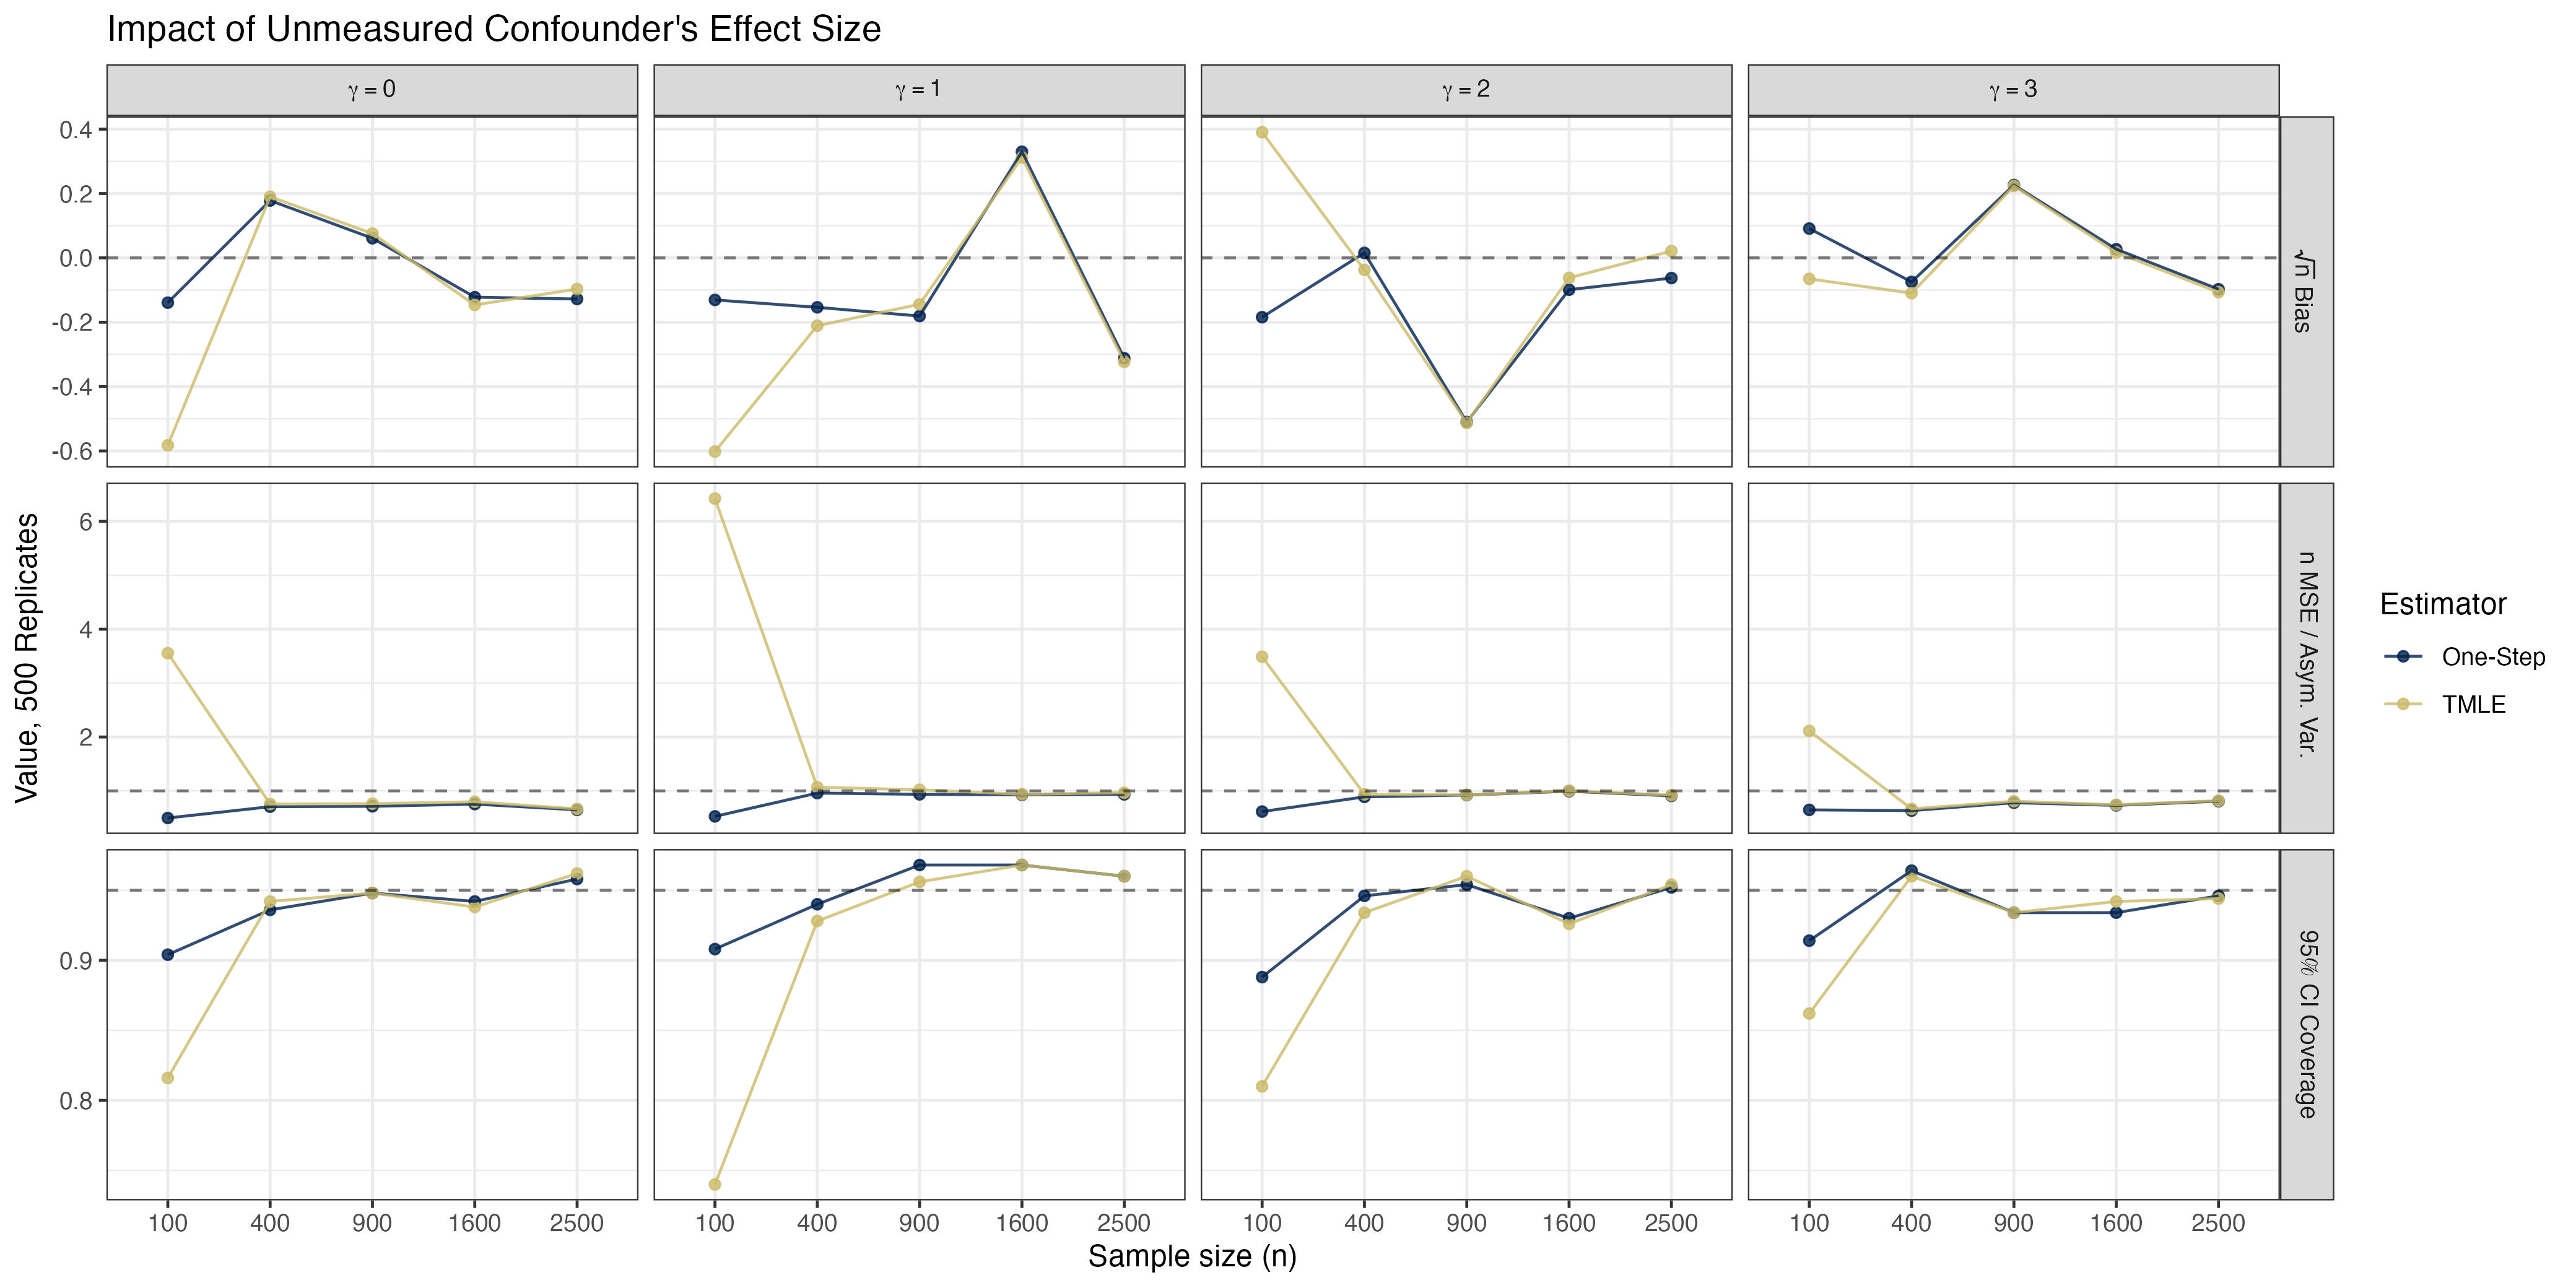
\includegraphics[width=0.295\textwidth]{figs/impact-unmeasured-conf-eff-size-sim.jpeg}
    \end{tikzfigure}
    \vspace{-1.5em}
  }

  \myblock{Conclusions}{
    Here are the important takeaways.
  }


  \mysmallblock{References}{
    \vspace{-3em}
    \bibliographystyle{unsrtnat}
    \bibliography{refs}
    \vspace{-1em}
  }


  \block[linewidth=0mm, bodyinnersep=5mm, roundedcorners=12]{}{
    {\small \textit{$^\ast$ indicates shared first-authorship}}
  }

\end{columns}

\end{document}
